%Theoretical Mechanics Homework_3
\documentclass[10pt,a4paper]{article}
\usepackage[UTF8]{ctex}
\usepackage{bm}
\usepackage{amsmath}
\usepackage{extarrows}
\usepackage{amsthm}
\usepackage{amssymb}
\usepackage{graphicx}
\usepackage{multirow}
\title{理论力学作业\_3}
\author{陈稼霖 \and 45875852}
\date{2018.11.2}
\begin{document}
\maketitle
\section*{Q1.}解:
以地面为静止参考系,以杆$OA$为绕定点$O$的转动参考系。

\noindent 点$C$的绝对速度为$\bm{v}$。

\noindent 点$C$的相对速度设为$\bm{v}'$(沿$\overrightarrow{OA}$方向)。

\noindent 杆$OA$的牵连速度为$\omega\times\overrightarrow{OC}$

\noindent 根据相对运动关系,有
\[
\bm{v} = \bm{v}' + \omega\times\overrightarrow{OC}
\]
做速度矢量图,注意到$\bm{v}' = 0$,在平行地面方向有
\[
v = \omega\frac{R}{\sin\theta}
\]
解得该瞬时杆的角速度
\[
\omega = \frac{v}{R}\sin\theta
\]
方向垂直纸面朝外。

\noindent 点$C$的绝对加速度为$\bm{a}$。

\noindent 点$C$的相对加速度设为$\bm{a}'$(沿$\overrightarrow{OA}$方向)。

\noindent 杆$OA$的牵连加速度为$\dot{\bm{\omega}}\times\overrightarrow{OC} - \omega^2\overrightarrow{OC}$。

\noindent 点$C$在转动参考系中的科里奥利加速度为$2\bm{\omega}\times\bm{v}' = 0$。

\noindent 根据相对运动关系,有
\[
\bm{a} = \bm{a}' + \dot{\bm{\omega}}\times\overrightarrow{OC} - \omega^2\overrightarrow{OC}
\]
做加速度矢量图,
在平行和垂直地面方向上分别有
\begin{align*}
&a = a'\sin\theta + \dot{\omega}\frac{R}{\sin\theta}\\
&0 = a'\cos\theta - \omega^2\frac{R}{\sin\theta}
\end{align*}
解得该瞬时杆的角加速度
\[
\dot{\omega} = \frac{a}{R}\sin\theta - \frac{v^2}{R^2}\sin^2\theta\tan\theta
\]
若$\dot{\omega} > 0$,则其方向垂直纸面朝外,否则其方向垂直纸面朝内。
\section*{Q2.}证明:
以炮弹发射点为原点,炮弹发射点处经线的切线为$x$轴(朝南为正方向),纬线的切线为$y$轴(朝东为正方向),垂直于地表的直线为$z$ 轴(由地心指向外为正方向),建立随地球转动的坐标系。设沿$x,y,z$轴正方向的单位矢量为$\bm{i},\bm{j},\bm{k}$。设炮弹在这一转动参考系中的坐标为$(x,y,z)$,速度为$\bm{v}' = \dot{x}\bm{i} + \dot{y}\bm{j} + \dot{z}\bm{k}$,加速度为$\bm{a}' = \ddot{x}\bm{i} + \ddot{y}\bm{j} + \ddot{z}\bm{k}$。 根据转动参考系中的牛顿第二定律,有
\[
m\bm{a}' = \bm{F} - mg\bm{k} - 2m\bm{\omega}\times\bm{v}'
\]
其中,由于在抛体运动中炮弹不受除重力外的任何力,故$\bm{F} = 0$; 地球的自转的角速度可表示为$\bm{\omega} = -\omega\cos\lambda\bm{i} + \omega\sin\lambda\bm{k}$,故
\[
\bm{\omega}\times\bm{v}' = -\omega\dot{y}\sin\lambda\bm{i} + \omega(\dot{x}\sin\lambda + \dot{z}\cos\lambda)\bm{j} - \omega\dot{y}\cos\lambda\bm{k}
\]
从而得到炮弹在$x,y,z$三个轴向上的运动微分方程为
\begin{equation}
\label{Q2DifferentialEquationofMotion}
\begin{split}
&m\ddot{x} = 2m\omega\dot{y}\sin\lambda\\
&m\ddot{y} = -2m\omega(\dot{x}\sin\lambda + \dot{z}\cos\lambda)\\
&m\ddot{z} = -mg + 2m\omega\dot{y}\cos\lambda
\end{split}
\end{equation}
上式积分对$t$积分一次并考虑到$t = 0$时,$x = 0, y = 0, z = 0, \dot{x} = 0, \dot{y} = V\cos\alpha, \dot{z} = V\sin\alpha$,得到
\begin{align*}
&\dot{x} = 2\omega y\sin\lambda\\
&\dot{y} = -2\omega(x\sin\lambda + z\cos\lambda) + V\cos\alpha\\
&\dot{z} = -gt + 2\omega y\cos\lambda + V\sin\alpha
\end{align*}
将上式回代入式(\ref{Q2DifferentialEquationofMotion}),得到
\begin{align*}
&\ddot{x} = 2\omega[-2\omega(x\sin\lambda + z\cos\lambda) + V\cos\alpha]\sin\lambda\\
&\ddot{y} = -2\omega[2\omega y\sin^2\lambda + (-gt + 2\omega y\cos\lambda + V\sin\alpha)\cos\lambda]\\
&\ddot{z} = -g + 2\omega[-2\omega(x\sin\lambda + z\cos\lambda) + V\cos\alpha]\cos\lambda
\end{align*}
由于$\omega$项极小,忽略$\omega^2$项和$\ddot{z}$式中的$\omega$项,得到
\begin{align*}
&\ddot{x} = 2\omega V\cos\alpha\sin\lambda\\
&\ddot{y} = 2\omega(gt - V\sin\alpha)\cos\lambda\\
&\ddot{z} = -g
\end{align*}
上式对$t$积分两次并考虑初始条件,得到
\begin{align*}
&x = \omega Vt^2\cos\alpha\sin\lambda\\
&y = \omega(\frac{1}{3}gt^3 - Vt^2\sin\alpha)\cos\lambda + Vt\cos\alpha\\
&z = -\frac{1}{2}gt^2 + Vt\sin\alpha
\end{align*}
当炮弹落地时,$z = 0$,解得
\[
t = \frac{2V\sin\alpha}{g}
\]
代入$x$式中得到横向偏移为
\[
d = x = \frac{4V^3}{g^2}\omega\sin\lambda\sin^2\alpha\cos\alpha
\]
\section*{Q3.}解:
如图(\ref{Q3}),设圆圈的圆心为$C$,$CO$和$CM$之间的夹角为$\theta$。
\begin{figure}[h]
\centering
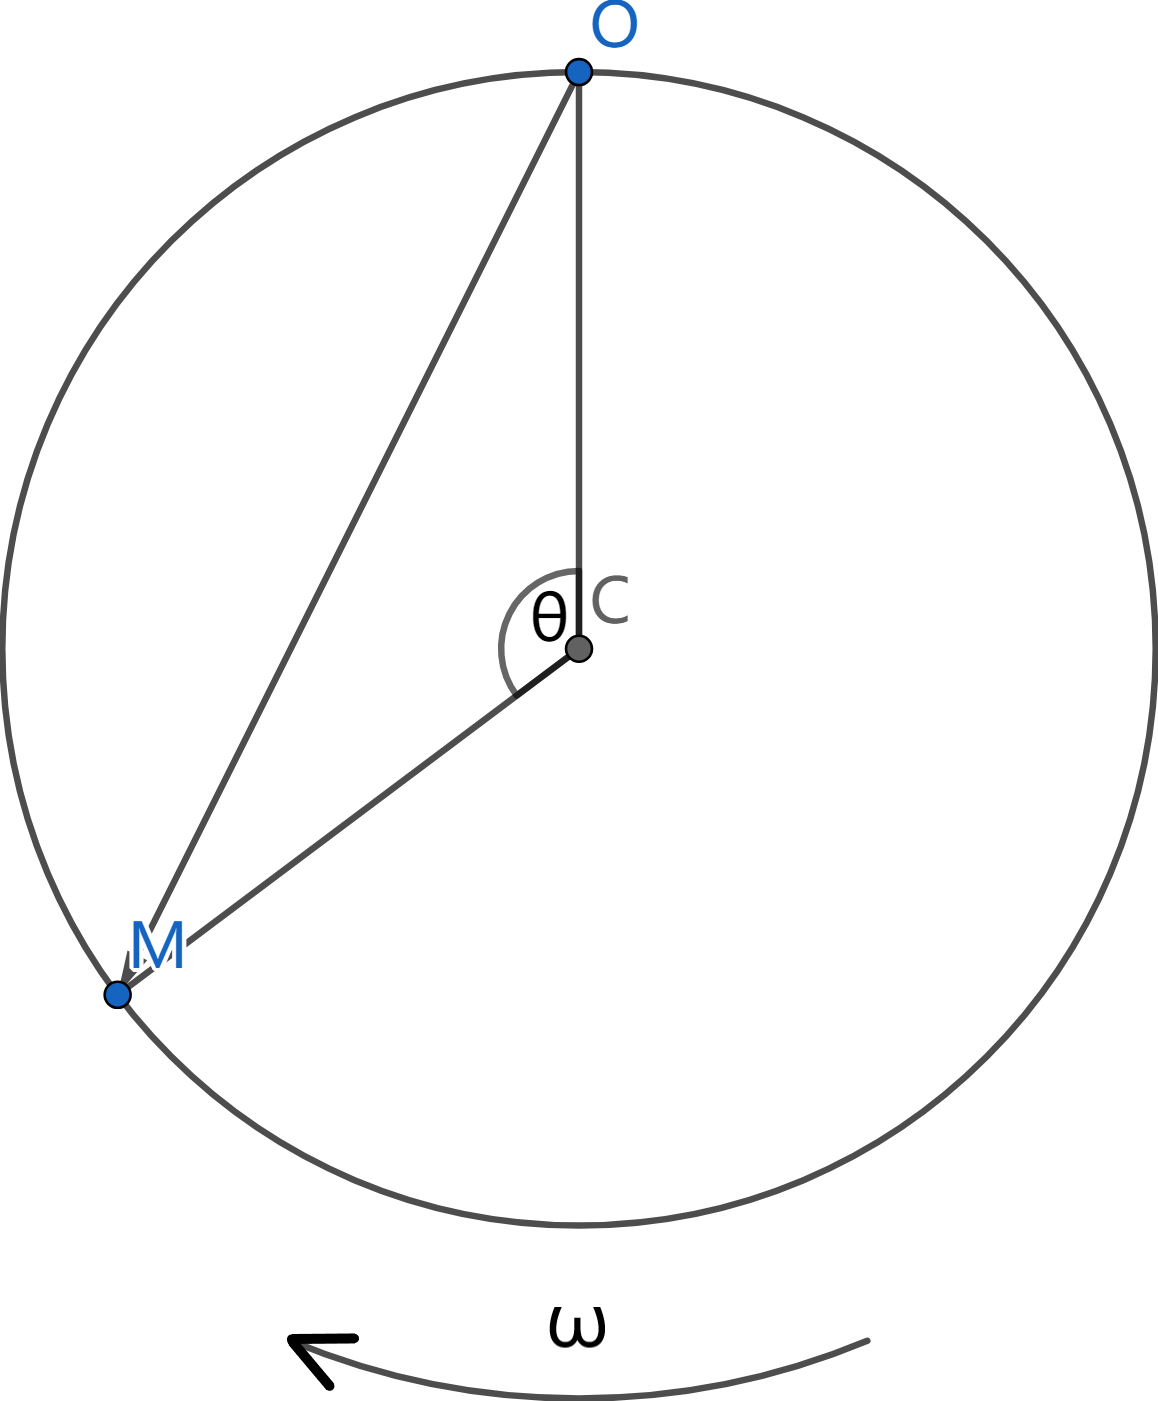
\includegraphics[scale=.15]{Homework_3Q3(marked).png}
\caption{Q3图}\label{Q3}
\end{figure}

在圆圈这一平面转动参考系中,对于小环,根据牛顿第二定律,有
\[
m\bm{a}' = \bm{F} + m\omega^2\overrightarrow{OM} - 2m\bm{\omega}\times\bm{v}'
\]
其中$\bm{a}'$为小环在转动参考系中的加速度,$\bm{F}$为小环受到的作用力,在题设条件下为圆圈对小环的支持力,垂直于圆圈的切线方向,$\bm{v}'$为小环对在转动参考系中的速度,垂直于圆圈的切线方向。故沿切线方向有
\begin{align*}
&ma_t = m\omega^2\cdot2a\sin\frac{\theta}{2}\cdot\cos\frac{\theta}{2}\\
&\Longrightarrow a_t = \omega^2a\sin\theta
\end{align*}
由于$a_t = a\ddot{\theta}$,故
\[
\ddot{\theta} = \omega^2\sin\theta
\]
\section*{Q4.}
\subsection*{(i)}解:
以$A$点为原点,$AC$所在直线为$x$轴,建立平面直角坐标系。设$B$ 点坐标为$(x_1,y_1)$,$D$点坐标为$(x_2,x_2)$,$E$点坐标为$(x_3,y_3)$。 根据虚功原理,机构的平衡条件为
\[
-W\delta y_1 + k(x_3 - x_2)\delta x_2 - k(x_3 - x_2)\delta x_3 = 0
\]
利用广义坐标$\angle BAC = \theta$表示各点坐标
\begin{align*}
&y_1 = (a + b)\sin\theta\\
&x_2 = a\cos\theta\\
&x_3 = (a + b)\cos\theta + b\cos\theta = (a + 2b)\cos\theta
\end{align*}
代入平衡条件得到
\begin{align*}
-W\delta((a + b)\sin\theta) + k((a + 2b)\cos\theta - a\cos\theta)\delta (b\cos\theta)&\\
- k((a + 2b)\cos\theta - a\cos\theta)\delta((a + 2b)\cos\theta)& = 0
\end{align*}
由于$\theta$为独立变量,故
\[
[-W(a + b) + 2kab\sin\theta]\cos\theta = 0
\]
解得机构的平衡位置为
\[
\theta = \arcsin\frac{W(a + b)}{2kab}
\]
此时各点坐标为$B((a + b)\cos\theta,(a + b\cos\theta)),C(2(a + b)\cos\theta,0),D(a\cos\theta,a\sin\theta),E((a + 2b)\cos\theta,a\sin\theta)$
\subsection*{(ii)}证明:
设杆的质心$C(x,y)$。根据虚功原理,杆的平衡条件为
\[
mg\delta y = 0
\]
又
\[
y = 2r\cos\alpha\sin\alpha - \frac{l}{2}\cos\alpha = r\sin2\alpha - \frac{l}{2}\cos\alpha
\]
代入平衡条件中得到
\[
mg\delta(r\sin2\alpha - \frac{l}{2}\cos\alpha) = mg(2r\cos2\alpha - \frac{l}{2}\cos\alpha)\delta\alpha = 0
\]
由于$\alpha$为独立变量,故
\begin{equation}
\label{Q4(ii)}
2r\cos2\alpha - \frac{l}{2}\cos\alpha = 0
\end{equation}
又
\begin{align*}
&\cos\alpha = \frac{c}{2r}\\
\Longrightarrow\cos2\alpha =& 2\cos^2\alpha - 1 = \frac{c^2 - 2r^2}{2r^2}
\end{align*}
代入式(\ref{Q4(ii)})中得到
\[
l = \frac{4(c^2 - 2r^2)}{c}
\]
\section*{Q5.}解:
以球心为原点,过原点竖直向上的直线为$z$轴,建立空间直角坐标系。根据虚功原理,平衡条件为
\[
m\bm{g}\delta\bm{r} = -mg\delta z = 0
\]
质点被限制在球面上运动,约束方程为
\[
f(x,y,z) = x^2 + y^2 + z^2 - a^2 = 0
\]
微分得
\[
2x\delta x + 2y\delta y + 2z\delta z = 0
\]
约束方程的微分与拉格朗日未定乘数$\lambda$相乘并加上平衡条件,有
\[
\lambda\cdot2x\delta x + \lambda\cdot2y\delta y + (-mg + \lambda\cdot2z)\delta z = 0
\]
由此得
\begin{align*}
&2\lambda x = 0\\
&2\lambda y = 0\\
&-mg + 2\lambda z = 0\\
&x^2 + y^2 + z^2 - a^2 = 0
\end{align*}
解得
\[
\left\{\begin{array}{l}
x = 0\\
y = 0\\
z = a\\
\lambda = \frac{mg}{2a}
\end{array}\right.
\text{或}
\left\{\begin{array}{l}
x = 0\\
y = 0\\
z = -a\\
\lambda = -\frac{mg}{2a}
\end{array}\right.
\]
约束力为
\[
\bm{R} = \lambda\nabla f = -m\bm{g}
\]
综上:质点的平衡位置有两个,分别为$(0,0,-a)$和$(0,0,a)$,在两点处的约束力大小均为$mg$,方向均为竖直向上。
\end{document}
